\section{Data Description and Additional Background}

This appendix gathers the material that would have slowed down the main text. It contains the background and diagnostics behind the empirical setup so that the main body can remain focused on the argument and interpretation.

\subsection{Descriptive role of the asset universe}

We did not select the assets for this dissertation at random. Each instrument represents a distinct component of the traditional financial system, which allows us to directly compare each of these components with Bitcoin. Bitcoin is the primary object of comparison and appears in each of them.

\begin{itemize}
    \item The S\&P 500 is used as a broad proxy for U.S. equity-market risk and general investor sentiment.
    \item The NASDAQ Composite captures a more growth-oriented and technology-heavy market segment, making it especially interesting in relation to crypto assets.
    \item Gold and silver ETFs represent precious-metal exposure, a domain frequently associated with hedging, inflation narratives, and safe-haven debates.
    \item The U.S. dollar index proxy reflects macro-defensive positioning and global dollar strength.
    \item Ethereum is included as a crypto-native comparison asset in order to contrast same-ecosystem dependency with cross-market dependency.
\end{itemize}

These assets differ in terms of criteria such as the investor base, degree of liquidity, sensitivity to general economic trends, and their significance to the economy as a whole. This diversity helps avoid conclusions based on an analysis of only a small portion of the market.

\subsection{Visual overview of the dataset}

Figure~\ref{fig:eda_prices_appendix} presents normalised price paths for the asset universe. The normalisation puts all series on a common starting point, which makes visible how different the underlying market trajectories are.

\begin{figure}[H]
    \centering
    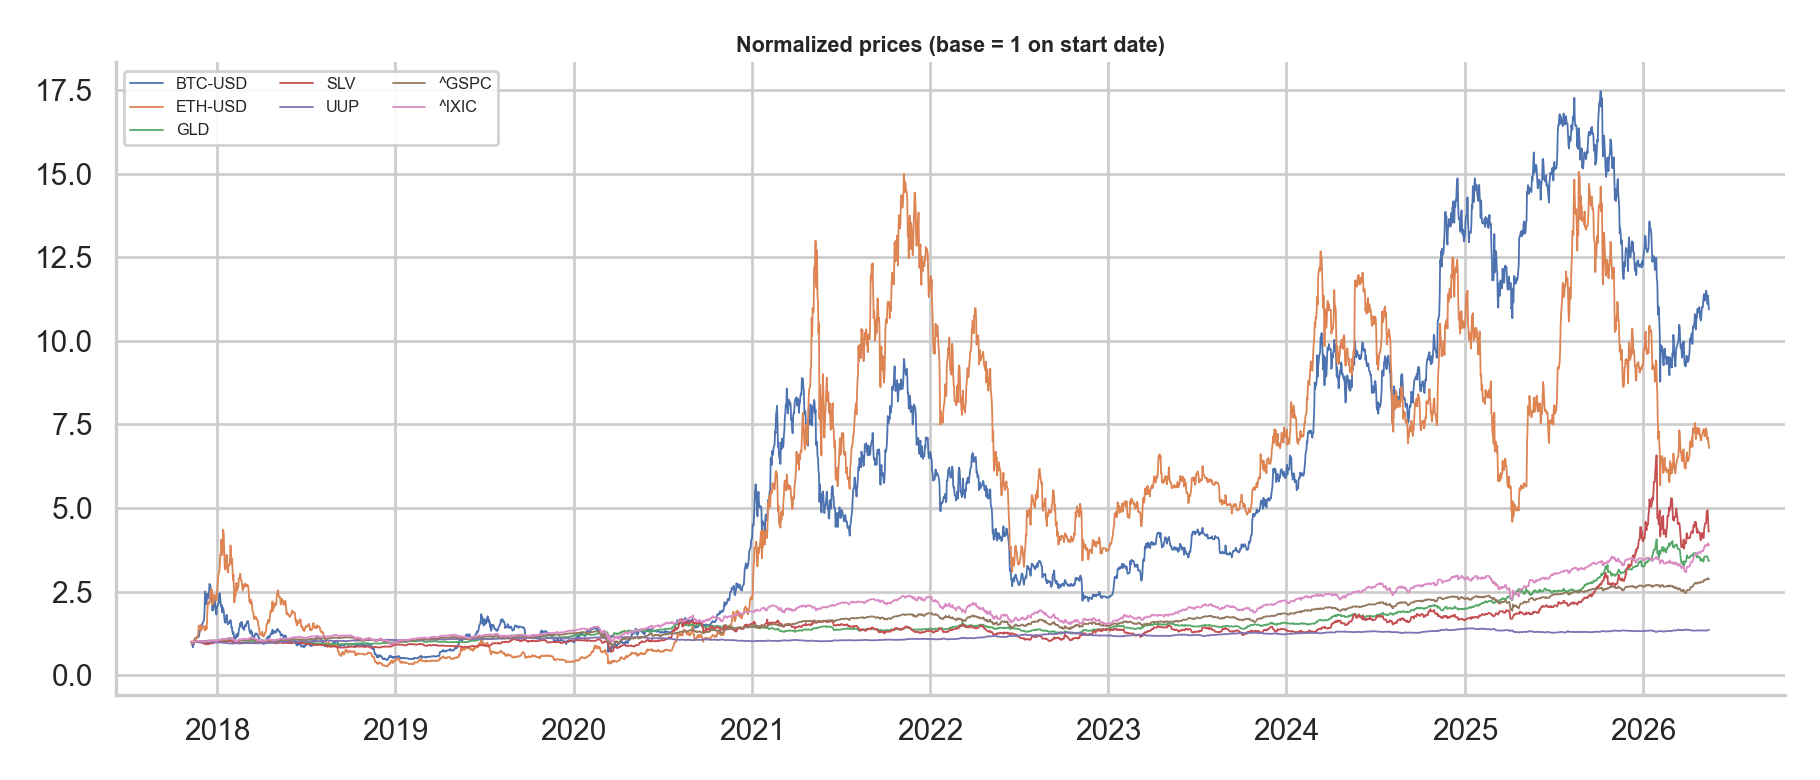
\includegraphics[width=0.95\textwidth]{../outputs/figures/eda_normalized_prices.png}
    \caption{Normalised prices of the assets included in the study.}
    \label{fig:eda_prices_appendix}
\end{figure}

Figure~\ref{fig:eda_vol_appendix} shows rolling volatility profiles. These reveal that Bitcoin and related crypto assets inhabit a much higher-volatility environment than the conventional asset set, which is one more reason to study the dependence dynamically.

\begin{figure}[H]
    \centering
    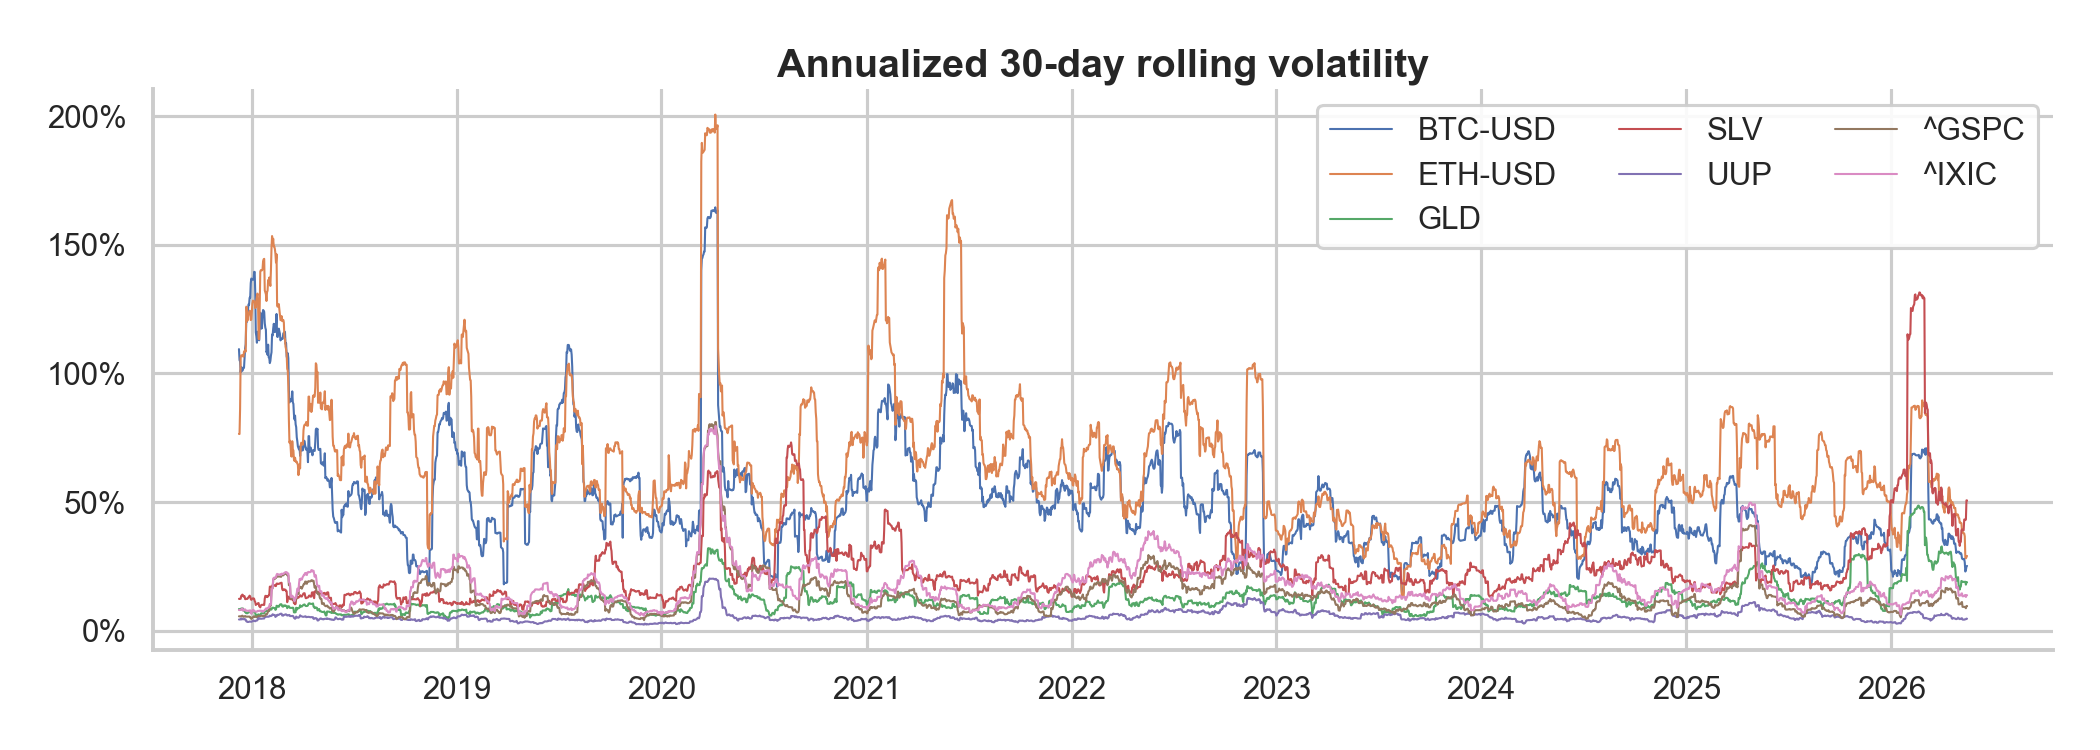
\includegraphics[width=0.95\textwidth]{../outputs/figures/eda_rolling_vol.png}
    \caption{Rolling volatility across the asset universe.}
    \label{fig:eda_vol_appendix}
\end{figure}

Figure~\ref{fig:eda_heatmap_appendix} provides the static correlation heatmap; the dynamic rolling-correlation structure is shown in the methodology chapter (Figure~\ref{fig:rolling_corr_all}). Together they motivate the main modelling choice of the thesis: static summaries are insufficient for describing the cross-market relations under study.

\begin{figure}[H]
    \centering
    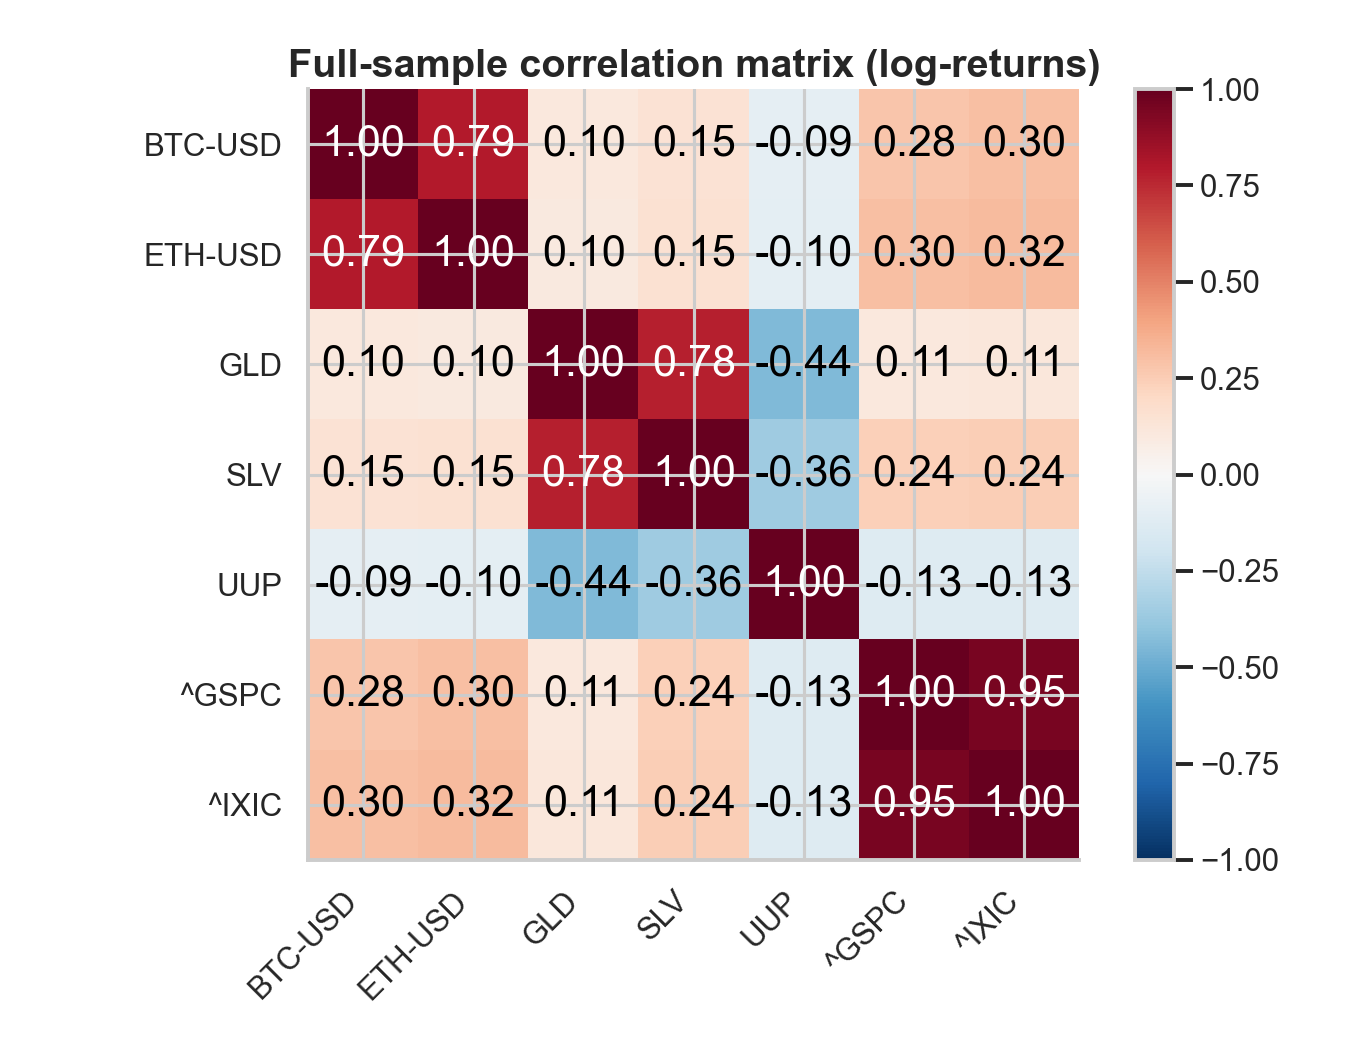
\includegraphics[width=0.85\textwidth]{../outputs/figures/eda_corr_heatmap.png}
    \caption{Static correlation heatmap of the return series.}
    \label{fig:eda_heatmap_appendix}
\end{figure}

\subsection{Dataset validation and quality diagnostics}

All price series are subjected to a systematic quality inspection before any modelling step. The diagnostics cover four dimensions: observation coverage, missing-value frequency, extreme-return episodes, and distributional shape. Table~\ref{tab:data_quality} summarises the per-ticker results.

\begin{table}[H]
\centering
\small
\caption{Data quality summary per ticker}
\label{tab:data_quality}
\resizebox{\textwidth}{!}{%
\begin{tabular}{lrrrrrrrrr}
\toprule
Ticker & First obs. & Last obs. & N & \% miss. & Gaps $>$2d & Zero ret. & Skew & Ex.Kurt & Ann.Vol (\%) \\
\midrule
BTC-USD & 2017-11-09 & 2026-05-16 & 3053 & 0.00 & 0 & 0 & -0.73 & 13.48 & 55.88 \\
ETH-USD & 2017-11-09 & 2026-05-16 & 3053 & 0.00 & 0 & 0 & -0.74 & 10.86 & 72.40 \\
GLD & 2017-11-09 & 2026-05-16 & 3053 & 0.00 & 0 & 920 & -0.87 & 13.63 & 13.88 \\
SLV & 2017-11-09 & 2026-05-16 & 3053 & 0.00 & 0 & 955 & -2.69 & 49.30 & 28.49 \\
UUP & 2017-11-09 & 2026-05-16 & 3053 & 0.00 & 0 & 1001 & -0.03 & 8.56 & 5.84 \\
\^{}GSPC & 2017-11-09 & 2026-05-16 & 3053 & 0.00 & 0 & 914 & -0.74 & 22.67 & 16.15 \\
\^{}IXIC & 2017-11-09 & 2026-05-16 & 3053 & 0.00 & 0 & 915 & -0.46 & 12.66 & 19.62 \\
\bottomrule
\end{tabular}
}
\end{table}

Figure~\ref{fig:dq_coverage} confirms that all seven tickers share an uninterrupted observation window from November 2017 to May 2026, with no gaps in coverage after alignment.

\begin{figure}[H]
    \centering
    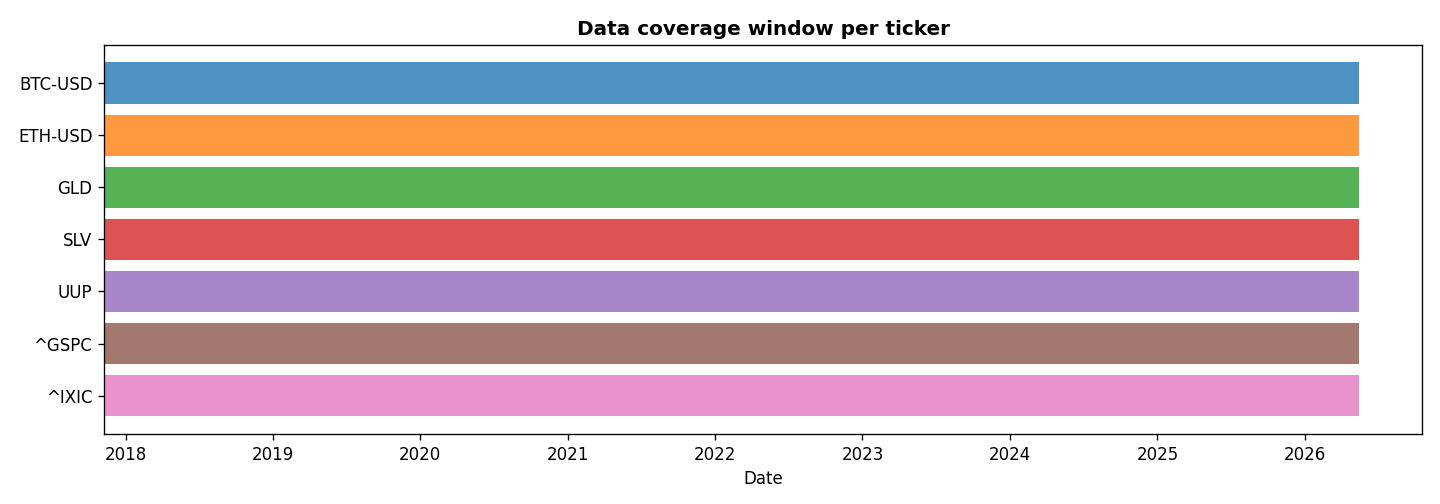
\includegraphics[width=0.88\textwidth]{../outputs/figures/fig_price_coverage.png}
    \caption{Observation coverage window per ticker. All assets share an identical aligned date range after the ETH-USD availability cutoff in November 2017.}
    \label{fig:dq_coverage}
\end{figure}

Figure~\ref{fig:dq_outliers} shows extreme return events ($|z\text{-score}| > 5\sigma$) for each asset. Bitcoin and Ethereum have the outliers with the largest absolute magnitude. This reflects the known fat-tailed pattern in crypto returns (excess kurtosis 13.5 for Bitcoin). These are not, however, the most extreme series in the sample. Silver has an excess kurtosis of 49.3 and the S\&P~500 has 22.7. These numbers are not directly comparable with the crypto ones because the moments for the five conventional assets are calculated using a return vector in which about 30\% of the entries are forced to zero for weekends. This makes the variance smaller and increases the standardised fourth moment. All five conventional assets have many zero-return days. This is not an ETF-specific issue. It happens because these five-day-a-week assets are matched to Bitcoin's seven-day schedule. The weekend gaps are filled with zeros, so every Saturday and Sunday has a forced zero return, while the crypto assets that trade continuously have no such zeros.

This calendar difference is a real limitation. On weekend days, a real Bitcoin return is matched with a zero conventional return. This makes the rolling correlation smaller. A further concern is that forward-filling could make the target more persistent. This is important because persistence is a major part of the results in Chapters~\ref{sec:results_overview} and~\ref{sec:discussion}. To check this directly, the 30-day Bitcoin--S\&P~500 rolling correlation was calculated using common trading days only. The 914 weekend and holiday rows were removed, and the persistence was compared with the full-calendar version. The persistence is essentially the same. It is even slightly higher without the weekend rows. The lag-1 autocorrelation of the Fisher-$z$ target is 0.977 with the seven-day calendar and 0.981 with trading days only. The naive ``tomorrow-equals-today'' $R^2$ is 0.954 versus 0.961. The same pattern is found for the 14-day and 90-day windows.

The forced weekend zeros therefore add some noise rather than creating artificial persistence. The main role of persistence is therefore not a result of the calendar choice. Using trading days only would be a useful refinement for future work, but it would not change the main findings. None of the detected outliers are data errors. They are genuine price events and are kept in the analysis.

\begin{figure}[H]
    \centering
    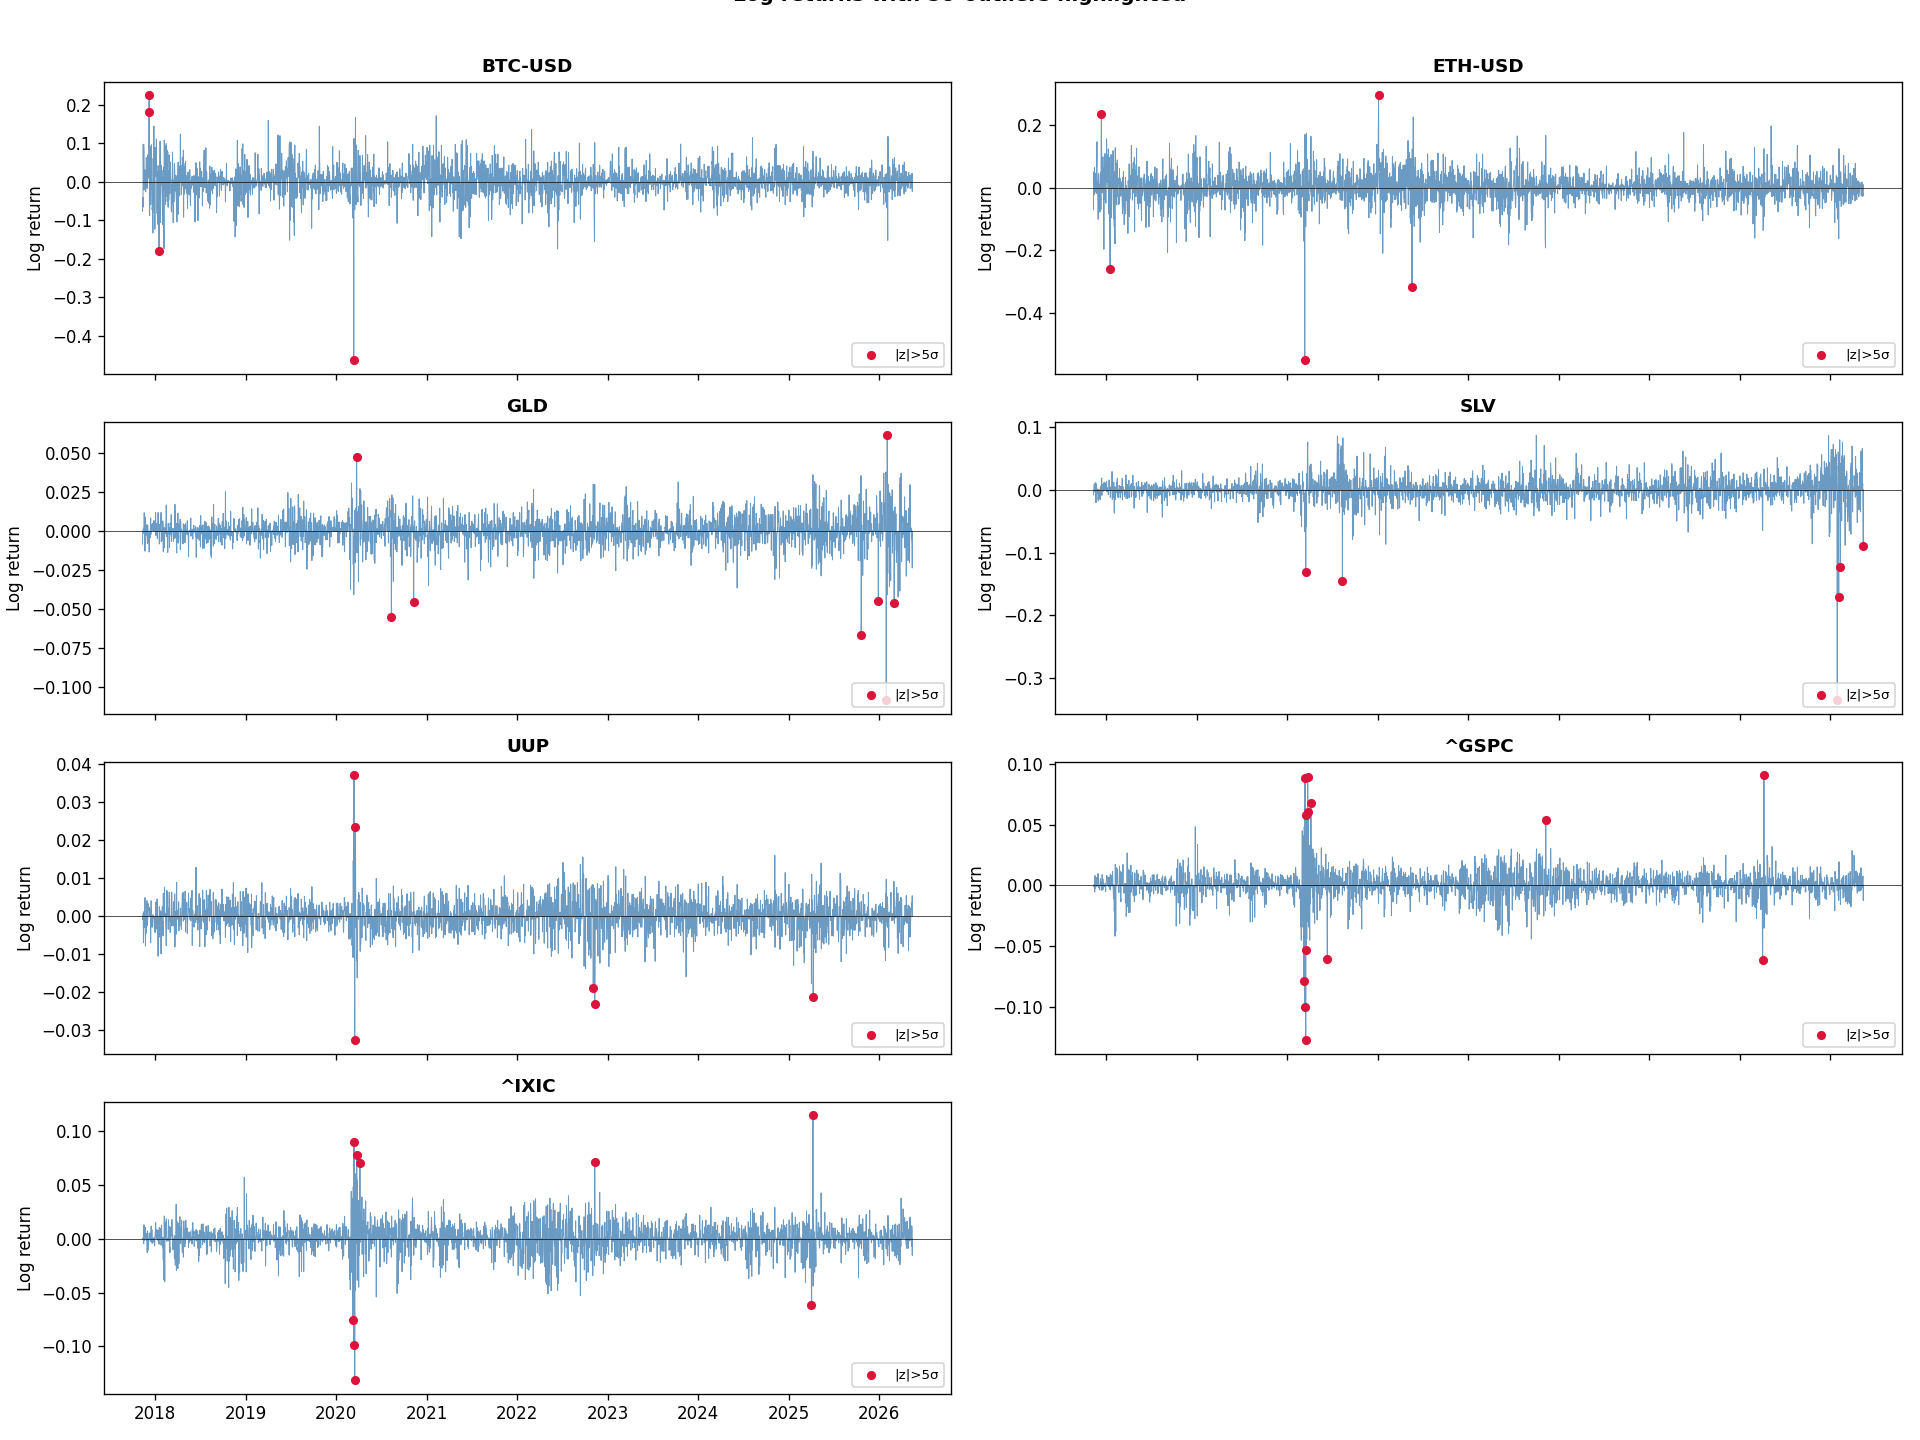
\includegraphics[width=0.95\textwidth]{../outputs/figures/fig_return_outliers.png}
    \caption{Log-return series with extreme observations ($|z|>5\sigma$) highlighted in red. Crypto assets exhibit sporadic but large outliers; conventional assets are more contained but not outlier-free.}
    \label{fig:dq_outliers}
\end{figure}

\subsection{Fisher-z transformation of the correlation target}

The rolling Pearson correlation $\rho_t$ is bounded on $(-1, 1)$ and exhibits variance compression near the boundaries. Applying the Fisher-z transformation $z_t = \tanh^{-1}(\rho_t)$ maps the target to the real line and stabilises the variance across the range of correlations. Figure~\ref{fig:eda_fisher} illustrates the distributional improvement for the representative Bitcoin--S\&P~500 pair at the 30-day window: the untransformed correlation distribution is left-skewed and bounded, while the Fisher-transformed version is more symmetric and approximately Gaussian.

\begin{figure}[H]
    \centering
    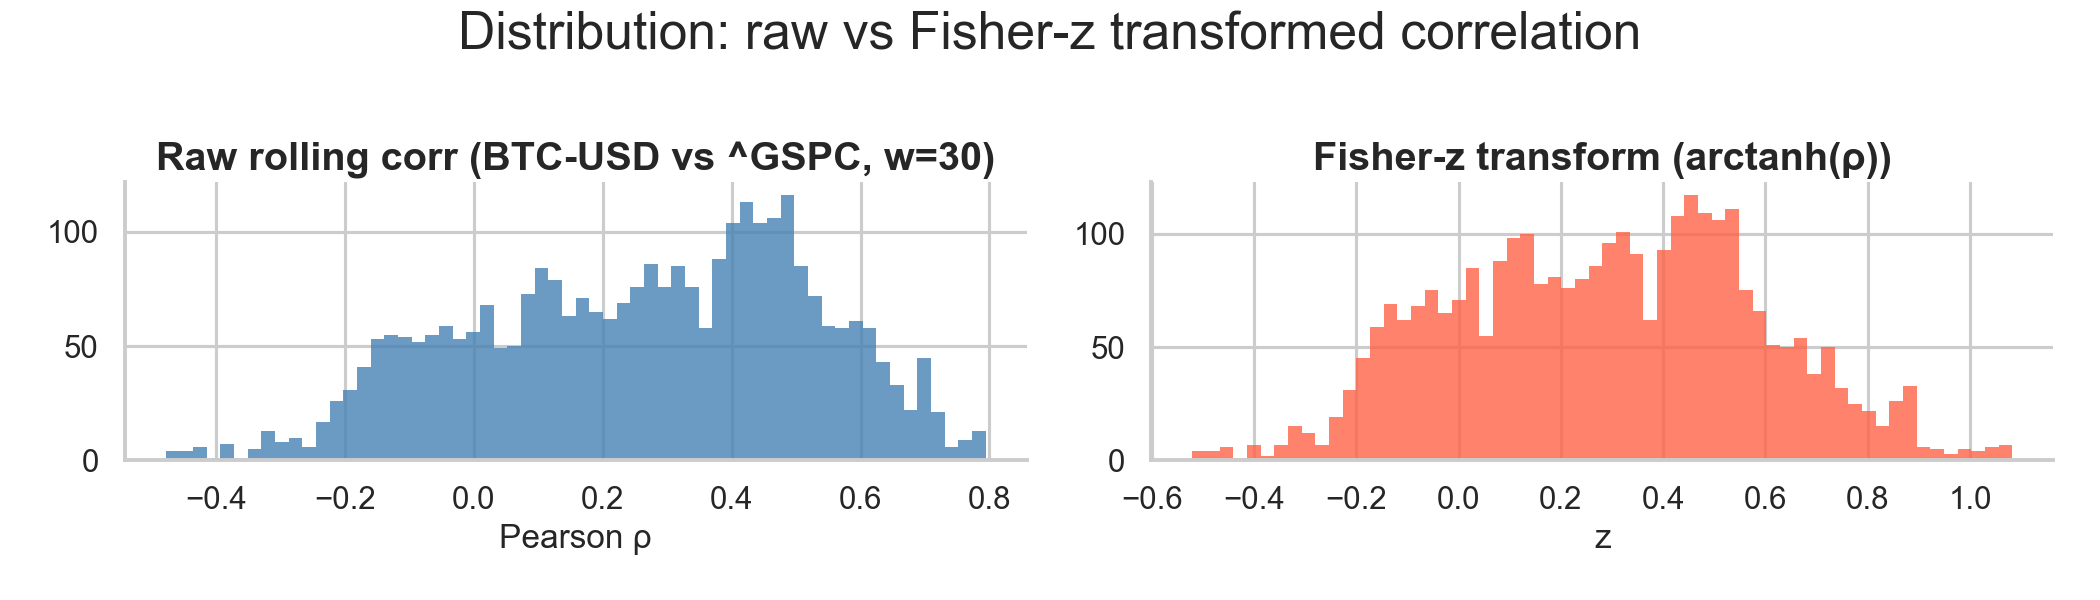
\includegraphics[width=0.88\textwidth]{../outputs/figures/eda_fisher_transform.png}
    \caption{Distribution of the 30-day rolling correlation before and after Fisher-z transformation for the Bitcoin--S\&P~500 pair. The transformation improves normality and removes boundary compression.}
    \label{fig:eda_fisher}
\end{figure}

\subsection{Why multiple rolling windows are used}

The thesis uses 14-, 30-, 60-, and 90-day windows because no single horizon is the right one. A short window reacts fast to recent shocks but is noisy; a long window is smoother and more persistent but slow to register a regime change. Running all four lets the analysis tease these effects apart.

The window choice turns out to shape the whole forecastability profile. Longer windows are easier to forecast because they are smoother --- but that success is almost entirely persistence. Shorter windows are noisier, yet more informative about local instability.

\subsection{Additional implementation remarks}

Each time the pipeline runs, the agreed-upon results are written to the \texttt{outputs/results}, \texttt{outputs/tables}, \texttt{outputs/figures}, and \texttt{outputs/predictions} folders. This promotes the reproducibility of results, but also makes it easier to write a report: since the tables and figures are taken directly from the code, the gap between conducting the experiment and writing the report is minimal.

The notebooks were designed in accordance with the development process, and they were not allowed to deviate from it. In the notebooks, the plots are easy to interpret, and the control metrics are selected reliably. The notebooks use auxiliary functions without making assumptions about the fragility of the trajectory. This is important in practice. Research notebooks often differ from the code used to obtain the results and become unreliable over time.

\subsection{Summary}

The conclusion is of a methodological nature: the environment studied here is heterogeneous, economically non-stationary, and sufficiently complex to justify treating the relationship as one that varies over time. The descriptive data confirm the modeling strategy outlined in the main text.
